\documentclass[12pt]{article}
\usepackage[utf8]{inputenc}
\usepackage[T1]{fontenc}
\usepackage{amsmath, amssymb, amsfonts, graphicx, hyperref, geometry, parskip, listings, caption}
\usepackage{breqn}
\usepackage{float}
\usepackage{color} % For listings syntax highlighting
\geometry{a4paper, margin=2.5cm}
\lstset{
    language=Python,
    basicstyle=\ttfamily\scriptsize,
    keywordstyle=\color{blue},
    stringstyle=\color{red},
    commentstyle=\color{green!60!black},
    showstringspaces=false,
    breaklines=true,
    breakatwhitespace=true,
    frame=single,
    xleftmargin=2mm,
    xrightmargin=2mm
}
\hyphenation{Uni-ver-sal Re-so-nance Mas-ter Equa-tion quan-tum-clas-si-cal hy-brid sys-tems Ap-pli-ca-tion Ca-te-go-ries for-mer-ly se-pa-rate equa-tions}

\title{\textbf{Resonance Master Equation -- Key to New Dimensions}}
\author{Adrian Zander -- \href{mailto:zander.adrian@gmx.de}{zander.adrian@gmx.de}}
\date{\today}

\begin{document}
\maketitle

\begin{abstract}
\begin{sloppypar}
This whitepaper presents a modular and unified framework for modeling physical systems through the lens of resonance. By introducing the Universal Resonance Master Equation, we encapsulate diverse phenomena ranging from classical lattice dynamics to quantum-classical hybrid systems. We reduce model complexity to a single generalized form governed by tunable parameters. Through a modular Python template, the framework enables simulation of phenomena such as solitons, stochastic responses, topological effects, and multi-scale resonance. Simulation snapshots included herein illustrate lattice wave propagation and soliton emergence. This unification of physical dynamics through resonance offers both theoretical elegance and practical applicability in a wide range of scientific and engineering contexts.
\end{sloppypar}
\end{abstract}

\clearpage

\section*{Introduction}
The Universal Resonance Model (URM) proposes that all physical phenomena can be understood as networks of coupled oscillations. This document provides a mathematical-physical foundation and corresponding numerical simulation strategies in Python.

\section*{Core Equation: Universal Resonance Master Equation}
\begin{dmath}
m \ddot{x}_{i,j} = k \Delta x_{i,j} - c \dot{x}_{i,j} - \alpha x_{i,j}^3 - \beta x_{i,j}^5 + q E_{i,j}(t) + \lambda \langle \hat{Q}_{i,j} \rangle + \gamma X_{i,j}(t) + \eta T_{i,j} + \xi \zeta_{i,j}(t) + F_{i,j}(t)
\end{dmath}

\subsection*{Meaning of Terms}
\begin{itemize}
\item $\Delta x_{i,j}$: Discrete Laplacian (lattice coupling)
\item $\alpha, \beta$: Nonlinearities (cubic, quintic)
\item $E_{i,j}(t)$: External classical field (e.g., electromagnetic)
\item $\langle \hat{Q}_{i,j} \rangle$: Quantum expectation value
\item $X_{i,j}(t)$: Macroscopic coupling (e.g., mean field amplitude)
\item $T_{i,j}$: Topological term (e.g., local defects)
\item $\zeta_{i,j}(t)$: Stochastic noise
\item $F_{i,j}(t)$: External driving (e.g., sinusoidal force)
\end{itemize}

\clearpage

\section*{Python: Modular Simulation Template}
\begin{lstlisting}[language=Python]
def external_field(i, j, t):
    return np.sin(0.1 * i + t)

def quantum_expectation(i, j, t):
    return np.sin(0.05 * i * j + t)

def macro_resonance(x):
    return np.mean(x)

def topological_term(i, j, x, N):
    term1 = abs(x[i, j] - x[(i + 1) % N, j])
    term2 = abs(x[i, j] - x[i, (j + 1) % N])
    return term1 + term2

def stochastic_noise():
    return np.random.normal(0, 1)
\end{lstlisting}

\clearpage

\section*{\small Application Categories (formerly separate equations)}

\subsection*{RNLE -- Resonant Nonlinear Lattice Equation}
$-\alpha x^3, -\beta x^5$: For classical nonlinear solid-state models.

\subsection*{FCLE -- Field-Coupled Lattice Equation}
$+ q\, E_{i,j}(t)$: Coupling to external fields.

\subsection*{MSCRE -- Multi-Scale Coupled Resonance}
$+ \gamma\, X_{i,j}(t)$: Feedback via macroscopic resonance.

\subsection*{QCRE -- Quantum-Coupled Resonance}
$+ \lambda\, \langle \hat{Q}_{i,j} \rangle$: Hybrid quantum-classical coupling.

\subsection*{TRE -- Topological Resonance Equation}
$+ \eta\, T_{i,j}$: Topological effects (e.g., edges, defects).

\subsection*{DQRE / DDRE -- Dissipative Quantum/Driven Resonance}
$+ \xi\, \zeta_{i,j}(t)$: Stochastic or environmental influences.

\section*{Conclusion}
All special cases are covered by tuning parameters in the master equation. This modular structure supports efficient and scalable implementation for exploring complex oscillator networks.

\begin{figure}[H]
\centering
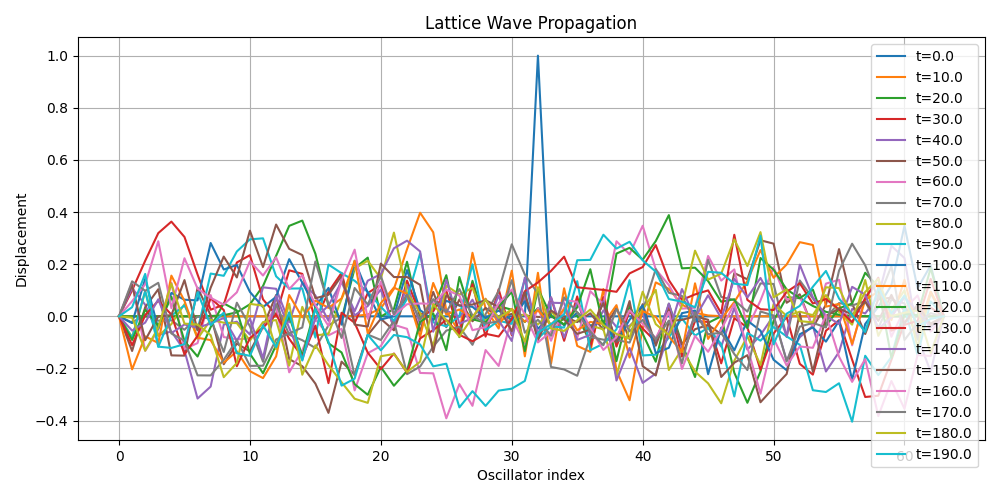
\includegraphics[width=0.8\textwidth]{lattice_wave_propagation.png}
\caption{Wellenpropagation im Gitter (Wave Propagation in the Lattice)}
\end{figure}

\begin{figure}[H]
\centering
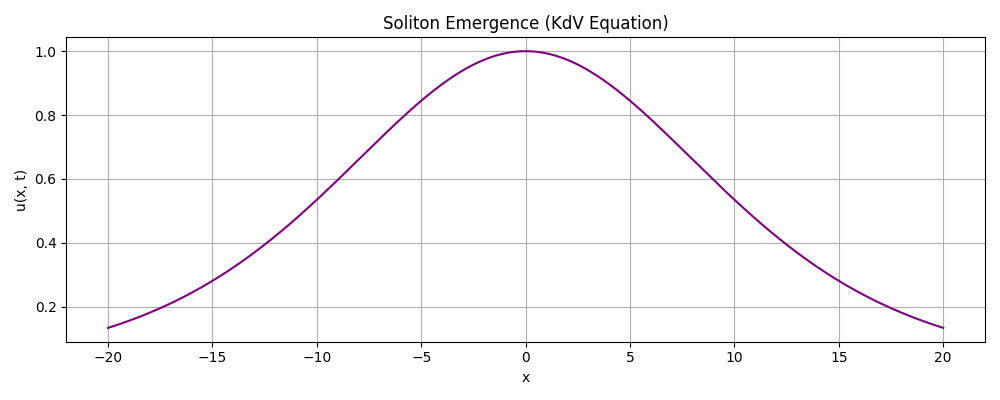
\includegraphics[width=0.8\textwidth]{soliton_emergence.png}
\caption{Solitonentstehung (Soliton Emergence)}
\end{figure}

\end{document}